\documentclass{ximera}

%\usepackage{todonotes}

\newcommand{\todo}{}

\usepackage{esint} % for \oiint
\ifxake%%https://math.meta.stackexchange.com/questions/9973/how-do-you-render-a-closed-surface-double-integral
\renewcommand{\oiint}{{\large\bigcirc}\kern-1.56em\iint}
\fi


\graphicspath{
  {./}
  {ximeraTutorial/}
  {basicPhilosophy/}
  {functionsOfSeveralVariables/}
  {normalVectors/}
  {lagrangeMultipliers/}
  {vectorFields/}
  {greensTheorem/}
  {shapeOfThingsToCome/}
  {dotProducts/}
  {partialDerivativesAndTheGradientVector/}
  {../productAndQuotientRules/exercises/}
  {../normalVectors/exercisesParametricPlots/}
  {../continuityOfFunctionsOfSeveralVariables/exercises/}
  {../partialDerivativesAndTheGradientVector/exercises/}
  {../directionalDerivativeAndChainRule/exercises/}
  {../commonCoordinates/exercisesCylindricalCoordinates/}
  {../commonCoordinates/exercisesSphericalCoordinates/}
  {../greensTheorem/exercisesCurlAndLineIntegrals/}
  {../greensTheorem/exercisesDivergenceAndLineIntegrals/}
  {../shapeOfThingsToCome/exercisesDivergenceTheorem/}
  {../greensTheorem/}
  {../shapeOfThingsToCome/}
  {../separableDifferentialEquations/exercises/}
  {vectorFields/}
}

\newcommand{\mooculus}{\textsf{\textbf{MOOC}\textnormal{\textsf{ULUS}}}}

\usepackage{tkz-euclide}
\usepackage{tikz}
\usepackage{tikz-cd}
\usetikzlibrary{arrows}
\tikzset{>=stealth,commutative diagrams/.cd,
  arrow style=tikz,diagrams={>=stealth}} %% cool arrow head
\tikzset{shorten <>/.style={ shorten >=#1, shorten <=#1 } } %% allows shorter vectors

\usetikzlibrary{backgrounds} %% for boxes around graphs
\usetikzlibrary{shapes,positioning}  %% Clouds and stars
\usetikzlibrary{matrix} %% for matrix
\usepgfplotslibrary{polar} %% for polar plots
\usepgfplotslibrary{fillbetween} %% to shade area between curves in TikZ
%\usetkzobj{all}
\usepackage[makeroom]{cancel} %% for strike outs
%\usepackage{mathtools} %% for pretty underbrace % Breaks Ximera
%\usepackage{multicol}
\usepackage{pgffor} %% required for integral for loops



%% http://tex.stackexchange.com/questions/66490/drawing-a-tikz-arc-specifying-the-center
%% Draws beach ball
\tikzset{pics/carc/.style args={#1:#2:#3}{code={\draw[pic actions] (#1:#3) arc(#1:#2:#3);}}}



\usepackage{array}
\setlength{\extrarowheight}{+.1cm}
\newdimen\digitwidth
\settowidth\digitwidth{9}
\def\divrule#1#2{
\noalign{\moveright#1\digitwidth
\vbox{\hrule width#2\digitwidth}}}




% \newcommand{\RR}{\mathbb R}
% \newcommand{\R}{\mathbb R}
% \newcommand{\N}{\mathbb N}
% \newcommand{\Z}{\mathbb Z}

\newcommand{\sagemath}{\textsf{SageMath}}


%\renewcommand{\d}{\,d\!}
%\renewcommand{\d}{\mathop{}\!d}
%\newcommand{\dd}[2][]{\frac{\d #1}{\d #2}}
%\newcommand{\pp}[2][]{\frac{\partial #1}{\partial #2}}
% \renewcommand{\l}{\ell}
%\newcommand{\ddx}{\frac{d}{\d x}}

% \newcommand{\zeroOverZero}{\ensuremath{\boldsymbol{\tfrac{0}{0}}}}
%\newcommand{\inftyOverInfty}{\ensuremath{\boldsymbol{\tfrac{\infty}{\infty}}}}
%\newcommand{\zeroOverInfty}{\ensuremath{\boldsymbol{\tfrac{0}{\infty}}}}
%\newcommand{\zeroTimesInfty}{\ensuremath{\small\boldsymbol{0\cdot \infty}}}
%\newcommand{\inftyMinusInfty}{\ensuremath{\small\boldsymbol{\infty - \infty}}}
%\newcommand{\oneToInfty}{\ensuremath{\boldsymbol{1^\infty}}}
%\newcommand{\zeroToZero}{\ensuremath{\boldsymbol{0^0}}}
%\newcommand{\inftyToZero}{\ensuremath{\boldsymbol{\infty^0}}}



% \newcommand{\numOverZero}{\ensuremath{\boldsymbol{\tfrac{\#}{0}}}}
% \newcommand{\dfn}{\textbf}
% \newcommand{\unit}{\,\mathrm}
% \newcommand{\unit}{\mathop{}\!\mathrm}
% \newcommand{\eval}[1]{\bigg[ #1 \bigg]}
% \newcommand{\seq}[1]{\left( #1 \right)}
% \renewcommand{\epsilon}{\varepsilon}
% \renewcommand{\phi}{\varphi}


% \renewcommand{\iff}{\Leftrightarrow}

% \DeclareMathOperator{\arccot}{arccot}
% \DeclareMathOperator{\arcsec}{arcsec}
% \DeclareMathOperator{\arccsc}{arccsc}
% \DeclareMathOperator{\si}{Si}
% \DeclareMathOperator{\scal}{scal}
% \DeclareMathOperator{\sign}{sign}


%% \newcommand{\tightoverset}[2]{% for arrow vec
%%   \mathop{#2}\limits^{\vbox to -.5ex{\kern-0.75ex\hbox{$#1$}\vss}}}
% \newcommand{\arrowvec}[1]{{\overset{\rightharpoonup}{#1}}}
% \renewcommand{\vec}[1]{\arrowvec{\mathbf{#1}}}
% \renewcommand{\vec}[1]{{\overset{\boldsymbol{\rightharpoonup}}{\mathbf{#1}}}}

% \newcommand{\point}[1]{\left(#1\right)} %this allows \vector{ to be changed to \vector{ with a quick find and replace
% \newcommand{\pt}[1]{\mathbf{#1}} %this allows \vec{ to be changed to \vec{ with a quick find and replace
% \newcommand{\Lim}[2]{\lim_{\point{#1} \to \point{#2}}} %Bart, I changed this to point since I want to use it.  It runs through both of the exercise and exerciseE files in limits section, which is why it was in each document to start with.

% \DeclareMathOperator{\proj}{\mathbf{proj}}
% \newcommand{\veci}{{\boldsymbol{\hat{\imath}}}}
% \newcommand{\vecj}{{\boldsymbol{\hat{\jmath}}}}
% \newcommand{\veck}{{\boldsymbol{\hat{k}}}}
% \newcommand{\vecl}{\vec{\boldsymbol{\l}}}
% \newcommand{\uvec}[1]{\mathbf{\hat{#1}}}
% \newcommand{\utan}{\mathbf{\hat{t}}}
% \newcommand{\unormal}{\mathbf{\hat{n}}}
% \newcommand{\ubinormal}{\mathbf{\hat{b}}}

% \newcommand{\dotp}{\bullet}
% \newcommand{\cross}{\boldsymbol\times}
% \newcommand{\grad}{\boldsymbol\nabla}
% \newcommand{\divergence}{\grad\dotp}
% \newcommand{\curl}{\grad\cross}
%\DeclareMathOperator{\divergence}{divergence}
%\DeclareMathOperator{\curl}[1]{\grad\cross #1}
% \newcommand{\lto}{\mathop{\longrightarrow\,}\limits}

% \renewcommand{\bar}{\overline}

\colorlet{textColor}{black}
\colorlet{background}{white}
\colorlet{penColor}{blue!50!black} % Color of a curve in a plot
\colorlet{penColor2}{red!50!black}% Color of a curve in a plot
\colorlet{penColor3}{red!50!blue} % Color of a curve in a plot
\colorlet{penColor4}{green!50!black} % Color of a curve in a plot
\colorlet{penColor5}{orange!80!black} % Color of a curve in a plot
\colorlet{penColor6}{yellow!70!black} % Color of a curve in a plot
\colorlet{fill1}{penColor!20} % Color of fill in a plot
\colorlet{fill2}{penColor2!20} % Color of fill in a plot
\colorlet{fillp}{fill1} % Color of positive area
\colorlet{filln}{penColor2!20} % Color of negative area
\colorlet{fill3}{penColor3!20} % Fill
\colorlet{fill4}{penColor4!20} % Fill
\colorlet{fill5}{penColor5!20} % Fill
\colorlet{gridColor}{gray!50} % Color of grid in a plot

\newcommand{\surfaceColor}{violet}
\newcommand{\surfaceColorTwo}{redyellow}
\newcommand{\sliceColor}{greenyellow}




\pgfmathdeclarefunction{gauss}{2}{% gives gaussian
  \pgfmathparse{1/(#2*sqrt(2*pi))*exp(-((x-#1)^2)/(2*#2^2))}%
}


%%%%%%%%%%%%%
%% Vectors
%%%%%%%%%%%%%

%% Simple horiz vectors
\renewcommand{\vector}[1]{\left\langle #1\right\rangle}


%% %% Complex Horiz Vectors with angle brackets
%% \makeatletter
%% \renewcommand{\vector}[2][ , ]{\left\langle%
%%   \def\nextitem{\def\nextitem{#1}}%
%%   \@for \el:=#2\do{\nextitem\el}\right\rangle%
%% }
%% \makeatother

%% %% Vertical Vectors
%% \def\vector#1{\begin{bmatrix}\vecListA#1,,\end{bmatrix}}
%% \def\vecListA#1,{\if,#1,\else #1\cr \expandafter \vecListA \fi}

%%%%%%%%%%%%%
%% End of vectors
%%%%%%%%%%%%%

%\newcommand{\fullwidth}{}
%\newcommand{\normalwidth}{}



%% makes a snazzy t-chart for evaluating functions
%\newenvironment{tchart}{\rowcolors{2}{}{background!90!textColor}\array}{\endarray}

%%This is to help with formatting on future title pages.
\newenvironment{sectionOutcomes}{}{}



%% Flowchart stuff
%\tikzstyle{startstop} = [rectangle, rounded corners, minimum width=3cm, minimum height=1cm,text centered, draw=black]
%\tikzstyle{question} = [rectangle, minimum width=3cm, minimum height=1cm, text centered, draw=black]
%\tikzstyle{decision} = [trapezium, trapezium left angle=70, trapezium right angle=110, minimum width=3cm, minimum height=1cm, text centered, draw=black]
%\tikzstyle{question} = [rectangle, rounded corners, minimum width=3cm, minimum height=1cm,text centered, draw=black]
%\tikzstyle{process} = [rectangle, minimum width=3cm, minimum height=1cm, text centered, draw=black]
%\tikzstyle{decision} = [trapezium, trapezium left angle=70, trapezium right angle=110, minimum width=3cm, minimum height=1cm, text centered, draw=black]


\title{Function Features}


\begin{document}

\begin{abstract}
extreme values
\end{abstract}
\maketitle





Functions are packages containing three sets: domain, codomain, and pairs.  The pairs connect the domain values to codomain values and it is this relationship we want to investigate.   \\


For us, the codomain is often $\mathbb{R}$ and so we often ignore this until it becomes important.  (There are many reasons for it to become important).  Thus, we often think of our real-valued functions as three sets: domain, range, and pairs. \\


We would like to know how the range values are affected by the domain values. \\


\begin{itemize}
\item We are interested in the function values - the range values.  But they are controlled by the domain values. \\
\item We ask questions about the function values, but the answers are in the domain.
\end{itemize}




\begin{idea}


$\blacktriangleright$ \textbf{\textcolor{purple!85!blue}{Where}} is the maximum value of the function? 

Translation: Which \textbf{\textcolor{purple!85!blue}{domain}} value results in the maximum value of the function? \\


$\blacktriangleright$ \textbf{\textcolor{purple!85!blue}{Where}} is the minimum value of the function? 

Translation: Which \textbf{\textcolor{purple!85!blue}{domain}} value results in the minimum value of the function? \\


\end{idea}








A graph provides a global view of all of the pairs, which reveals many of the patterns, features, and characteristics we seek.   

However, we must separate the graph from the function.  The graph helps us answer the questions, but the graph doesn't hold the answers.  The answers are in the domain and range.  The answers are not the points in the graph.  The answers are the numbers in the domain and range.



\begin{center}

\textbf{\textcolor{blue!55!black}{The answers are not the points in the graph.}} \\

\textbf{\textcolor{blue!55!black}{The answers are the numbers in the domain and range.}}

\end{center}






\begin{explanation} \textbf{Video: Two Types of Questions}

[ Click on the arrow to the right to expand the video. ]
\begin{expandable} 

\begin{center}
\youtube{nMK4bo1Ad8g}
\end{center}

\end{expandable}
\end{explanation}








The graph displays patterns in its points.  These patterns help us analyze the function which has values in the range connected to numbers in the domain.




\subsection*{Maximum}



\begin{definition} \textbf{\textcolor{green!50!black}{Maximum}} 


Let $f$ be a function defined on the domain $D$.

Then $M$ is the \textbf{maximum value} of $f$ on $D$ if    


\begin{itemize}
\item There exists $d \in D$, such that $f(d) = M$.   i.e., $M$ has to be a function value \\

\item $f(d) \leq M$ for all $d \in D$. i.e., all function values are less than or equal to $M$. 

\end{itemize}


If there is no such $M$, then $f$ has no maximum value.

\end{definition}



\begin{observation}
The maximum value is visually encoded in the highest point on the graph of the function.  The second coordinate is the maximum value and the first coordinate is the domain number where the maximum occurs.
\end{observation}










\begin{example}

Below is the graph of $y=f(x)$.  

\begin{image}
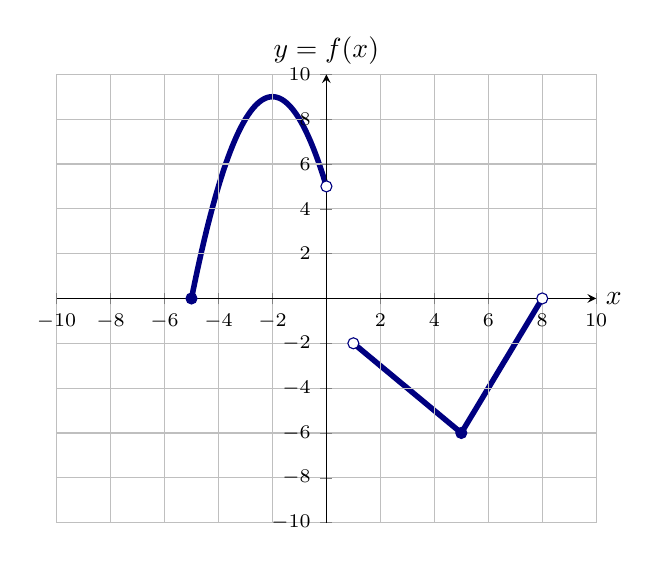
\begin{tikzpicture} 
  \begin{axis}[
            domain=-10:10, ymax=10, xmax=10, ymin=-10, xmin=-10,
            axis lines =center, xlabel=$x$, ylabel={$y=f(x)$},
            grid = both, 
            ytick={-10,-8,-6,-4,-2,2,4,6,8,10}, 
            xtick={-10,-8,-6,-4,-2,2,4,6,8,10},
            yticklabels={$-10$,$-8$,$-6$,$-4$,$-2$,$2$,$4$,$6$,$8$,$10$}, 
            xticklabels={$-10$,$-8$,$-6$,$-4$,$-2$,$2$,$4$,$6$,$8$,$10$},
            ticklabel style={font=\scriptsize},
            every axis y label/.style={at=(current axis.above origin),anchor=south},
            every axis x label/.style={at=(current axis.right of origin),anchor=west},
            axis on top
          ]
          
          \addplot [line width=2, penColor, smooth,samples=100,domain=(-5:0)] ({x},{(x+5)*(1-x)});
          \addplot [line width=2, penColor, smooth,samples=100,domain=(1:5)] ({x},{-x-1});
          \addplot [line width=2, penColor, smooth,samples=100,domain=(5:8)] ({x},{2*x-16});

          \addplot [color=penColor,fill=white,only marks,mark=*] coordinates{(0,5) (1,-2) (8,0)};
          \addplot [color=penColor,only marks,mark=*] coordinates{(-5,0) (5,-6)};


           

  \end{axis}
\end{tikzpicture}
\end{image}



\begin{question}

The highest point on the graph of $f$ is


\begin{multipleChoice}
\choice {$(-5,0)$}
\choice [correct]{$(-2,9)$}
\choice {$(0,5)$}
\choice {$(-1,-2)$}
\choice {$(5,-6)$}
\choice {$(8,0)$}
\end{multipleChoice}
\end{question}


\begin{question}
The maximum value of $f$ is $\answer{9}$, which occurs at $\answer{-2}$.
\end{question}







\end{example}










\begin{example}

Below is the graph of $y=g(t)$.  

\begin{image}
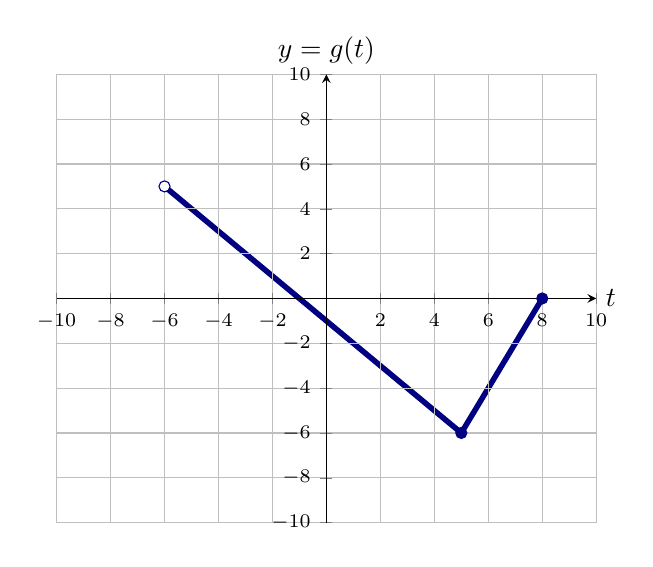
\begin{tikzpicture} 
  \begin{axis}[
            domain=-10:10, ymax=10, xmax=10, ymin=-10, xmin=-10,
            axis lines =center, xlabel=$t$, ylabel={$y=g(t)$},
            grid = both, 
            ytick={-10,-8,-6,-4,-2,2,4,6,8,10}, 
            xtick={-10,-8,-6,-4,-2,2,4,6,8,10},
            yticklabels={$-10$,$-8$,$-6$,$-4$,$-2$,$2$,$4$,$6$,$8$,$10$}, 
            xticklabels={$-10$,$-8$,$-6$,$-4$,$-2$,$2$,$4$,$6$,$8$,$10$},
            ticklabel style={font=\scriptsize},
            every axis y label/.style={at=(current axis.above origin),anchor=south},
            every axis x label/.style={at=(current axis.right of origin),anchor=west},
            axis on top
          ]
          

          \addplot [line width=2, penColor, smooth,samples=100,domain=(-6:5)] ({x},{-x-1});
          \addplot [line width=2, penColor, smooth,samples=100,domain=(5:8)] ({x},{2*x-16});

          \addplot [color=penColor,fill=white,only marks,mark=*] coordinates{(-6,5)};
          \addplot [color=penColor,only marks,mark=*] coordinates{(5,-6) (8,0)};


           

  \end{axis}
\end{tikzpicture}
\end{image}



There is no highest point on the graph.  Therefore, $g$ has no maximum value.

\end{example}


































\subsection*{Minimum}



\begin{definition} \textbf{\textcolor{green!50!black}{Minimum}} 


Let $f$ be a function defined on the domain $D$.

Then $M$ is the \textbf{minimum value} of $f$ on $D$ if    


\begin{itemize}
\item There exists $d \in D$, such that $f(d) = M$.   i.e., $M$ has to be a function value \\

\item $f(d) \geq M$ for all $d \in D$. i.e., all function values are greater than or equal to $M$. 

\end{itemize}


If there is no such $M$, then $f$ has no minimum value.

\end{definition}



\begin{observation}
The minimum value is visually encoded in the lowest point on the graph of the function.  The second coordinate is the minimum value and the first coordinate is the domain number where the minimum occurs.
\end{observation}










\begin{example}

Below is the graph of $y=f(x)$.  

\begin{image}
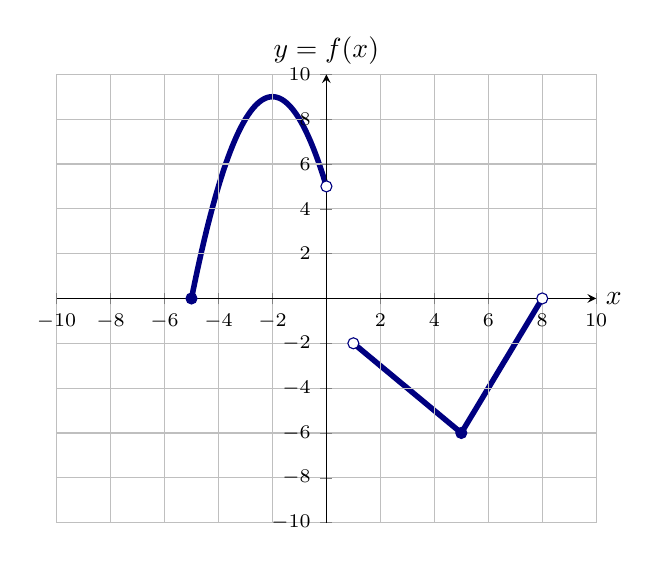
\begin{tikzpicture} 
  \begin{axis}[
            domain=-10:10, ymax=10, xmax=10, ymin=-10, xmin=-10,
            axis lines =center, xlabel=$x$, ylabel={$y=f(x)$},
            grid = both, 
            ytick={-10,-8,-6,-4,-2,2,4,6,8,10}, 
            xtick={-10,-8,-6,-4,-2,2,4,6,8,10},
            yticklabels={$-10$,$-8$,$-6$,$-4$,$-2$,$2$,$4$,$6$,$8$,$10$}, 
            xticklabels={$-10$,$-8$,$-6$,$-4$,$-2$,$2$,$4$,$6$,$8$,$10$},
            ticklabel style={font=\scriptsize},
            every axis y label/.style={at=(current axis.above origin),anchor=south},
            every axis x label/.style={at=(current axis.right of origin),anchor=west},
            axis on top
          ]
          
          \addplot [line width=2, penColor, smooth,samples=100,domain=(-5:0)] ({x},{(x+5)*(1-x)});
          \addplot [line width=2, penColor, smooth,samples=100,domain=(1:5)] ({x},{-x-1});
          \addplot [line width=2, penColor, smooth,samples=100,domain=(5:8)] ({x},{2*x-16});

          \addplot [color=penColor,fill=white,only marks,mark=*] coordinates{(0,5) (1,-2) (8,0)};
          \addplot [color=penColor,only marks,mark=*] coordinates{(-5,0) (5,-6)};


           

  \end{axis}
\end{tikzpicture}
\end{image}




\begin{question}

The lowest point on the graph of $f$ is


\begin{multipleChoice}
\choice {$(-5,0)$}
\choice {$(-2,9)$}
\choice {$(0,5)$}
\choice {$(-1,-2)$}
\choice [correct]{$(5,-6)$}
\choice {$(8,0)$}
\end{multipleChoice}
\end{question}


\begin{question}
The minimum value of $f$ is $\answer{-6}$, which occurs at $\answer{5}$.
\end{question}







\end{example}










\begin{example}

Below is the graph of $y=H(k)$.  

\begin{image}
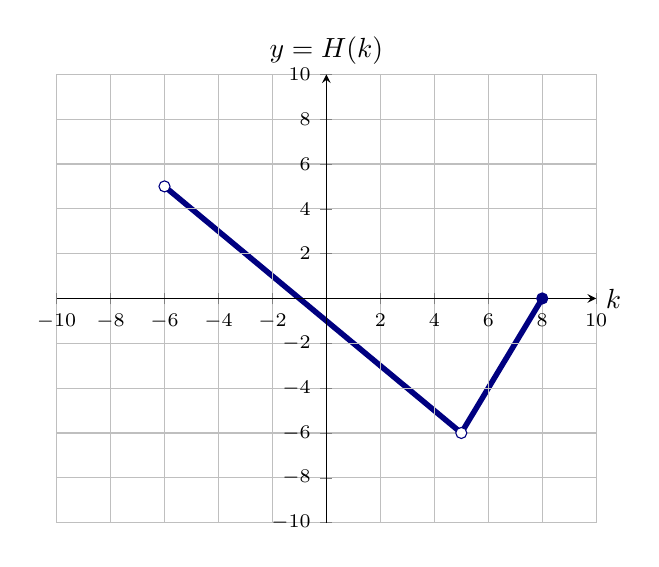
\begin{tikzpicture} 
  \begin{axis}[
            domain=-10:10, ymax=10, xmax=10, ymin=-10, xmin=-10,
            axis lines =center, xlabel=$k$, ylabel={$y=H(k)$},
            grid = both, 
            ytick={-10,-8,-6,-4,-2,2,4,6,8,10}, 
            xtick={-10,-8,-6,-4,-2,2,4,6,8,10},
            yticklabels={$-10$,$-8$,$-6$,$-4$,$-2$,$2$,$4$,$6$,$8$,$10$}, 
            xticklabels={$-10$,$-8$,$-6$,$-4$,$-2$,$2$,$4$,$6$,$8$,$10$},
            ticklabel style={font=\scriptsize},
            every axis y label/.style={at=(current axis.above origin),anchor=south},
            every axis x label/.style={at=(current axis.right of origin),anchor=west},
            axis on top
          ]
          

          \addplot [line width=2, penColor, smooth,samples=100,domain=(-6:5)] ({x},{-x-1});
          \addplot [line width=2, penColor, smooth,samples=100,domain=(5:8)] ({x},{2*x-16});

          \addplot [color=penColor,fill=white,only marks,mark=*] coordinates{(-6,5) (5,-6)};
          \addplot [color=penColor,only marks,mark=*] coordinates{(8,0)};


           

  \end{axis}
\end{tikzpicture}
\end{image}



There is no lowest point on the graph.  Therefore, $H$ has no minimum value.

\end{example}



















\begin{center}
\textbf{\textcolor{green!50!black}{ooooo-=-=-=-ooOoo-=-=-=-ooooo}} \\

more examples can be found by following this link\\ \link[More Examples of Function Graphs]{https://ximera.osu.edu/csccmathematics/precalculus1/precalculus1/functionGraphs/examples/exampleList}

\end{center}



\end{document}
